%%%%%%%%%%%%%%%%%%%%%%%%%%%%%%%%%%%%%%%%%%%%%%%%%%%%%%%%%%%%%%%%%%%%%%%%%%%%%%%
\section{An Example Workflow: Local Running}
\label{sec:localrunning}
%%%%%%%%%%%%%%%%%%%%%%%%%%%%%%%%%%%%%%%%%%%%%%%%%%%%%%%%%%%%%%%%%%%%%%%%%%%%%%%
Hello, World! jobs are all very well, but we're guessing your workflows
are more complicated than a printing out a simple, if polite, greeting.
We're now going to demonstrate the capabilities of Ganga and the
\textbf{CernVM-File System} (CernVM-FS, or CVMFS) for running jobs with
input data, remotely-managed software, and output data.

%=============================================================================
\subsection{An aside: what is the CernVM-FS?}
\label{an-aside-what-is-the-cernvm-fs}
%=============================================================================
The \href{http://cernvm.cern.ch/portal/startcvmfs}{CernVM File System}~\cite{CVMFS2015}
is ``\emph{a network file system based on HTTP and optimized to deliver
software in a fast, scalable, and reliable way}''. It was developed to
solve the problem of installing and maintaining the software used by all
of the different particle physics communities involved with work at
\href{https://cern.ch}{CERN}. Simply put, systems with the CernVM-FS
installed have instant access to a given community's software
repositories via the command line. This means it can be used:

\begin{itemize}
\tightlist
\item
  by community members working on university computing clusters outside
  of CERN;
\item
  by Worker Nodes (WN) anywhere on the grid where the repository is
  supported;
\item
  by CernVM Virtual Machines.
\end{itemize}

You've already used CVMFS to run Ganga itself. But it can be used to
host your own software that will run anywhere on the Grid (or, indeed,
anywhere with access to CVMFS).

The example workflow we'll use comes from the
\href{http://researchinschools.org/CERN/}{CERN@school research
programme}. We'll take some raw particle detector data in ASCII format,
turn it into some pretty images of detected particles using the Python
\texttt{matplotlib} software, and retrieve the frame information and
images as output.

%=============================================================================
\subsection{The workflow itself}
\label{the-workflow-itself}
%=============================================================================
The workflow here is pretty straightforward:

\begin{itemize}
\tightlist
\item \textbf{Input}: raw
detector data from a \href{http://medipix.web.cern.ch}{Timepix hybrid
silicon pixel detector}. These ASCII text files represent the data (and
detector settings) recorded by a Timepix detector during a background
measurement reading. The dataset we use here is hosted on the web at
\href{http://figshare.com}{FigShare}. We will download a \texttt{zip}
file containing the data and upload it with our job.
\item \textbf{Processing}: the data is processed with a Python script in the
CERN@school CVMFS repository called \texttt{process-frames.py}. This
script in turn uses Python modules (both custom and standard) that are
also hosted on and sourced from CVMFS.
\item \textbf{Output}:
\texttt{process-frames.py} produces a log file, a JSON containing
information about the processed data frames, and a directory of images
representing the particles detected in each frame.
\end{itemize}

We will create a workflow in Ganga that uploads the input data we've
downloaded from FigShare, process it on our local machine, compress the
images into a single \texttt{tar} archive, and retrieve the log file,
JSON file, and \texttt{tar} archive as output.

%=============================================================================
\subsection{Getting the input data}
\label{getting-the-input-data}
%=============================================================================
In your working directory, which we will associate with the environment
variable \texttt{\$WORKINGDIR}, download the dataset as follows:

\begin{Shaded}
\begin{Highlighting}[]
\NormalTok{$ }\KeywordTok{export} \OtherTok{WORKINGDIR=$PWD}
\NormalTok{$ }\KeywordTok{cd} \OtherTok{$WORKINGDIR}
\NormalTok{$ }\KeywordTok{wget} \NormalTok{http://files.figshare.com/2600426/CERNatschool_backgroundrad_dataset.zip}
\NormalTok{$ }\KeywordTok{unzip} \NormalTok{CERNatschool_backgroundrad_dataset.zip}
\NormalTok{$ }\KeywordTok{rm} \NormalTok{CERNatschool_backgroundrad_dataset.zip}
\NormalTok{$ }\KeywordTok{ls}
\KeywordTok{B06-W0212}  \NormalTok{E09-W0092  README.md}
\end{Highlighting}
\end{Shaded}

\begin{infobox}{Data and jobs}
\emph{We could actually get our grid job to do this as part of the job. Or we
could tell our job to use input data that is already hosted on a grid
storage element. For simplicity, though, we will upload the data we have
just downloaded to our working directory with our job.}
\end{infobox}

We'll see how this is uploaded with the job below.

%=============================================================================
\subsection{Writing the executable}
\label{writing-the-executable}
%=============================================================================
With our \emph{Hello, World!} job(s), we used the built-in executable
\texttt{echo} to print a simple string. This workflow will use the shell
script below, \texttt{run.sh}, that contains the commands we want our
job to execute.

\begin{verbatim}
$ vim run.sh
$ chmod a+x run.sh
$ cat run.sh
#!/bin/bash
#
# Add the Python packages from the CERN@school CVMFS
# repository to the PYTHONPATH environment variable.
export PYTHONPATH=/cvmfs/cernatschool.egi.eu/lib/python2.6/site-packages/: \\
/cvmfs/cernatschool.egi.eu/lib64/python2.6/site-packages/:$PYTHONPATH
#
# Add CERN@school libraries to the LD_LIBRARY_PATH.
export LD_LIBRARY_PATH=/cvmfs/cernatschool.egi.eu/lib/: \\
/cvmfs/cernatschool.egi.eu/lib64/: \\
/cvmfs/cernatschool.egi.eu/lib64/atlas:$LD_LIBRARY_PATH
#
# Add CERN@school libraries to the PATH.
export PATH=/cvmfs/cernatschool.egi.eu/lib64/:/cvmfs/cernatschool.egi.eu/lib/: \\
/cvmfs/cernatschool.egi.eu/lib64/atlas:$PATH
#
# Unzip the uploaded input data.
unzip CERNatschool_backgroundrad_dataset.zip
#
# Run the CVMFS-hosted Python script on the data.
python /cvmfs/cernatschool.egi.eu/code/particle-rate-plotter/process-frames.py \\
$1 ./.
#
# Compress the images ready for retrieval.
tar -cvf output_images.tar PNG/
\end{verbatim}

You should make \texttt{run.sh} in your \texttt{\$WORKINGDIR} by copying
and pasting the above into your favourite text editor.

\begin{warningbox}{Executable scripts}
\emph{Don't forget to make the script executable with the}
\code{chmod}
\emph{command.}
\end{warningbox}

%=============================================================================
\subsection{Preparing the job}
\label{creating-configuring-and-submitting-the-job}
%=============================================================================
We'll use Ganga's \texttt{execfile} functionality to create, configure,
and submit our job with a short Python script called
\texttt{local\_job.py}, listed with explanatory comments below:

\begin{verbatim}
$ vim local_job.py # Copy and paste away!
$ cat local_job.py
## The Ganga job.
j = Job()

# Name the job.
j.name = "CERN@school_local_01"

# Tell Ganga it's running an executable: run.sh
j.application = Executable()
j.application.exe = File('run.sh')

# run.sh takes one argument - the dataset directory.
j.application.args = ['B06-W0212/2014-04-02-150255/']

# Specifiy which local files to upload with the job.
j.inputfiles = [ LocalFile('CERNatschool_backgroundrad_dataset.zip') ]

# Specify which files should be downloaded as output from the job.
j.outputfiles = [ LocalFile('frames.json'), \\
LocalFile('log_process-frames.log'), LocalFile('output_images.tar') ]
j.submit()
\end{verbatim}

You can then run this within Ganga using the \texttt{execfile} command
as before:

\begin{Shaded}
\begin{Highlighting}[]
\KeywordTok{Ganga} \NormalTok{In [X]: execfile(}\StringTok{'local_job.py'}\NormalTok{)}
\NormalTok{[}\KeywordTok{...} \NormalTok{job output messages ...]}
\end{Highlighting}
\end{Shaded}

\begin{warningbox}{Location location location}
\emph{Make sure you are running Ganga from}
\code{\$WORKINGDIR}
\emph{so that it can find}
\code{local\_job.py}.
\end{warningbox}

You can monitor the status of the job as before with the \texttt{jobs}
command. As the job is actually doing some work now, you may be able to
see the job assume the \texttt{running} status.

%=============================================================================
\subsection{Getting the job output}
\label{getting-the-job-output}
%=============================================================================
Once the job has finished, you can view the output of the text files as
before with the \texttt{peek} command:

\begin{Shaded}
\begin{Highlighting}[]
\KeywordTok{Ganga} \NormalTok{In [X]: j=jobs(X)}
\KeywordTok{Ganga} \NormalTok{In [X]: j.peek(}\StringTok{'log_process-frames.log'}\NormalTok{)}
\KeywordTok{INFO}\NormalTok{:root: * Creating directory }\StringTok{'././PNG'}\NormalTok{...}
\KeywordTok{INFO}\NormalTok{:root:}
\KeywordTok{INFO}\NormalTok{:root:* Found 60 datafiles.}
\end{Highlighting}
\end{Shaded}

To view the images you've created, you'll need to find where they have
been downloaded to on your local machine. If the job ID was ``1'', you
can do this with:

\begin{Shaded}
\begin{Highlighting}[]
\KeywordTok{Ganga} \NormalTok{In [X]: j = jobs(1)}
\KeywordTok{Ganga} \NormalTok{In [X]: j.outputdir}
\KeywordTok{Ganga} \NormalTok{Out [X]: }\StringTok{'/home/alovelace/gangadir/workspace/alovelace/LocalXML/1/output/'}
\end{Highlighting}
\end{Shaded}

\begin{Shaded}
\begin{Highlighting}[]
\NormalTok{$ }\KeywordTok{cd} \OtherTok{$WORKINGDIR}
\NormalTok{$ }\KeywordTok{cp} \NormalTok{/home/alovelace/gangadir/workspace/alovelace/LocalXML/1/output/output_images.tar \\\\}
\NormalTok{output_images.tar}
\NormalTok{$ }\KeywordTok{tar} \NormalTok{-xvf output_images.tar}
\KeywordTok{PNG/}
\KeywordTok{PNG/E09-W0092_2014-04-02-143123.png}
\NormalTok{[}\KeywordTok{...}\NormalTok{]}
\KeywordTok{PNG/E09-W0092_2014-04-02-142120.png}
\end{Highlighting}
\end{Shaded}

You can view these images with the following command, which will bring
up the Eye Of Gnome image viewer (assuming you have it installed on your
local machine). Use the arrow keys to move through the frames of data.

\begin{Shaded}
\begin{Highlighting}[]
\NormalTok{$ }\KeywordTok{eog} \NormalTok{PNG/ }\KeywordTok{&}
\end{Highlighting}
\end{Shaded}

So there we have it - we've run a (rather simple) workflow on our local
machine using Ganga. But here's the thing: to move this workflow (and,
indeed, most workflows) to the grid, we only need to do three things:

\begin{enumerate}
\def\labelenumi{\arabic{enumi}.}
\tightlist
\item
  Configure the job to use the GridPP DIRAC backend;
\item
  Put our input data on the grid and configure our job to use this;
\item
  Configure the job to write the output data to the grid.
\end{enumerate}

2) and 3) take a bit more work, but are optional (it really depends on
your input and output data as to what actually \emph{needs} to go on
the grid. But once you're setup for grid running, 1) only takes a
single line in your job configuration script:

\begin{Shaded}
\begin{Highlighting}[]
\KeywordTok{j.backend}\NormalTok{=Dirac()}
\end{Highlighting}
\end{Shaded}

Ganga does the rest. Does that sound good? Let's get you
\hyperref[sec:onthegrid]{set up on the grid then}.

%=============================================================================
\subsection{Checklist}
\label{sec:localrunning-checklist}
%=============================================================================

\begin{itemize}
\tightlist
\item
  I can create, configure, and submit a local job that uses
  local-sourced data as input and software hosted on CVMFS using Ganga;
\item
  I can view the output logs from my local job with the \texttt{peek}
  command;
\item
  I can find and retrieve the output of my local job using the
  \texttt{outputdir} command in Ganga.
\end{itemize}


%=============================================================================
\subsection{Testing}
\label{an-example-workflow-local-running---testing}
%=============================================================================

\begin{itemize}
\tightlist
\item
  \textbf{Successful running of the CERN@school example job}: Once you
  have run and retrieved the images from the example job, the first
  frame image should look something like that shown in
  Figure~\ref{fig:localrunningframe}.
\end{itemize}

%
\begin{figure}[htbp]
  \centering
  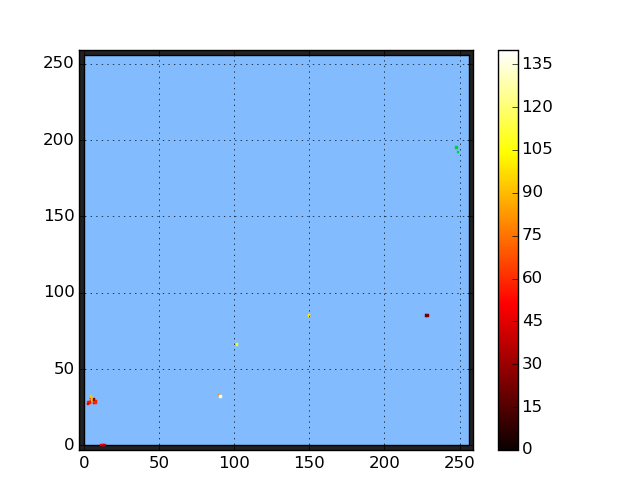
\includegraphics[width=0.7\textwidth]{assets/images/frame.png}
  \caption[The example output from the CERN@school job.]
  {\label{fig:localrunningframe}The example output from the CERN@school job.}
\end{figure}
%

For reference, that's a beta particle in the bottom left corner, and
five gammas in the rest of the frame! You can also find the source code
on the
\href{http://github.com/CERNatschool/particle-rate-plotter}{CERN@school
GitHub page}.

